\documentclass[11pt]{article}
\usepackage{url}
\usepackage{graphicx,DCCN2018_en}

\pagestyle{fancy}
\fancyhead{}
\fancyfoot{}

\usepackage[utf8]{inputenc}
\linespread{1.0}

\usepackage{amsmath}
\usepackage{placeins}

\makeatletter
\fancyhead[RO]{\small DCCN 2018\\ {17-21 September 2018}}
\fancyhead[LO]{\small Todor Balabanov, Ivan Blagoev, Kristina Dineva \\ Self Rising Tri Layers MLP for Time Series Forecasting}

\c@page=1
       
\makeatother

\title{Self Rising Tri Layers MLP for Time Series Forecasting}

\author[1]{\small T.D. Balabanov}
\author[1]{\small I.I. Blagoev}
\author[1]{\small K.I. Dineva}

\affil[1]{\footnotesize Institute of Information and Communication Technologies, Bulgarian Academy of Sciences, acad. Georgi Bonchev Str, block 2, office 514, 1113 Sofia, Bulgaria}

\email{todorb@iinf.bas.bg, i.blagoev@iit.bas.bg, k.dineva@iit.bas.bg}

\begin{document}

\udc{004.93}

{\let\newpage\relax\maketitle}

\vskip -1.5em

\footnotetext{This work was supported by private funding of Velbazhd Software LLC.}

\begin{abstract}
Time series forecasting is an attractive and heavily researched area. A very popular approach in this field is the usage of artificial neural networks. Some artificial neural network are oriented to deep learning as training algorithm. In this study instead of hidden layers number extension the size of input layer of tri layers multilayer perceptron is extended. The network starts with 1-1-1 topology. The input layer rise to n, according the size of input time series. In parallel hidden layer goes to m by application of pruning algorithm. Achieved topology n-m-1 is trained with classical backpropagation of the error.
\keywords{data mining, time series forecasting, artificial neural networks}
\end{abstract}

\section{Introduction} \label{Introduction}

There are numerous techniques applied in the field of times series forecasting \cite{atanasova01}. Artificial neural networks are one technique which is very successfully applied for such forecasting. Time series are values measured in the time by keeping strict order of the measurements (time-value pairs) \cite{balabanov01}. In most cases measurement interval is fixed, but expectations are also possible. The idea in time series is that values are not independent in time. Values are related in such way that future values are dependent from the past values. Forecasting problem is defined as - by knowing past values to do a prediction for the future values. In order such forecasting to be successful prediction model construction is needed. Artificial neural networks are one of the proven models in time series forecasting. Initially artificial neural networks were inspired by biological neural systems. First appearance of artificial neural networks was in the middle of 20th century \cite{balabanov02}. The most commonly used artificial neural networks are oriented weighted graphs. Nodes of the graph are called neurons. The links between the neurons have weights and these weights are the core of the information presented in the network. Artificial neural networks are working in two common modes - training and operation. The training mode is executed as an optimization task in which weights in the network should be modified in such way in which the network will learn the training patterns best. There are a lot of training algorithms developed during last four decades, but the most popular one is the backpropagation of the error. Backpropagation of the error is an exact numerical method and it is the prefered training method in this study. The idea is a minimization of the total neural network error achieved during processing of all training examples. The gradient of the total error is used for weights updating as direction of the update and the magnitude of the update. The way in which links between neurons are organized is common for the artificial neural network topology. There are a lot of different topologies widely investigated in the literature, like generalized nets \cite{tashev01} or deep learning neural networks. When the time series are too noise the input information can be filtered with Kalman filter for example \cite{alexandrov01}. 

In this study the main idea used into deep learning neural networks is reverted and instead of hidden layers number rising the size of the input and the hidden layers are extended during the neural network training. Extension of the input layer is related with the fact that each time series rise by appearance of a new measurement. The the goal of the training is the size of the input layer to get as big as the size of the full time series. 

The paper is organized as follows: Section \ref{Introduction} introduces the problem; Section \ref{Model Proposition} presents a model and optimization approach; Section \ref{Experiments and Results} gives experiment details; Section \ref{Conclusion} concludes and some further ideas for research are pointed.

\section{Model Proposition} \label{Model Proposition}

Conditionally the time series is divided to past and future. The values supplied into the input of the artificial neural network are called lag and they are subset of the past values nearest to the future values. The values obtained in the output of the artificial neural network are the prediction and they are compared with the subset of the future values called lead. As artificial neural network base, for the model proposed, multilayer perceptron is used with input, one hidden and output layers. 

In the proposed model set of artificial neural sub-networks is used and sub-networks are merged into a general artificial neural network. The smallest artificial neural sub-network has 1-1-1 topology (Fig. \ref{fig:pic01}-left). The network is trained with examples which input has only single value. The goal in the model is a forecast for only one value ahead in time. That is why all sub-networks have only single output. Fig. \ref{fig:pic01}-left shows only 3 intermediate examples of the training. All 29 input values are supplied as training examples to resilient backpropagation training. Training stops on certain epsilon level for total neural network error change.

\begin{figure}[ht!]
   \centering
     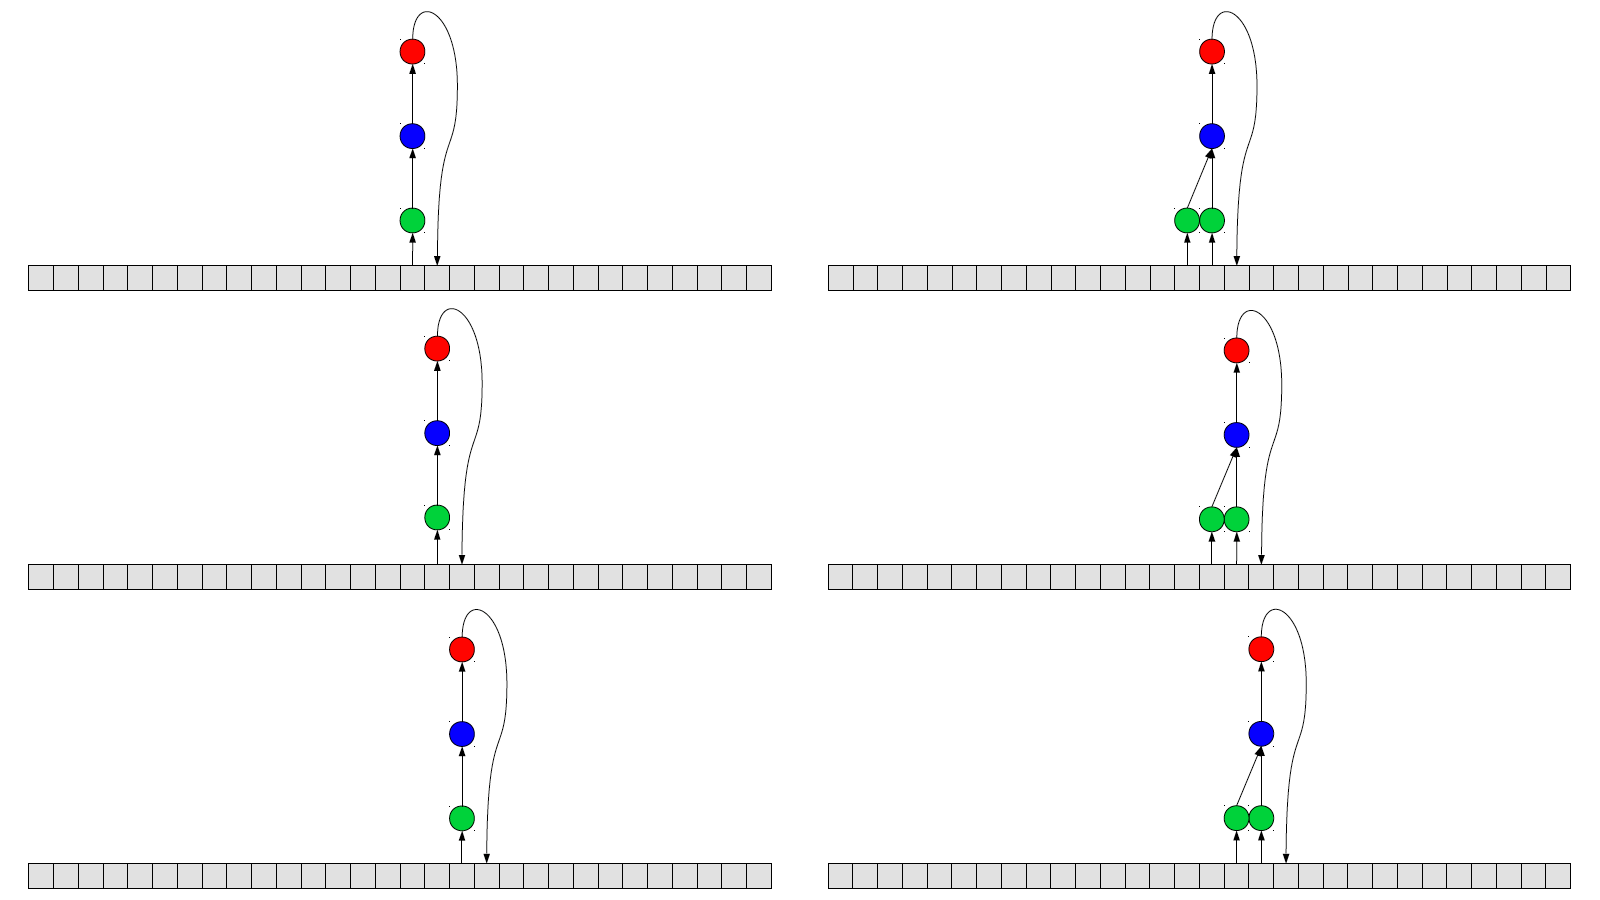
\includegraphics[width=0.8\textwidth]{pic01}
    \caption {Training of artificial neural sub-networks with 1-1-1 topology (left) and 2-1-1 topology (right).}
\label{fig:pic01}
\end{figure}
\FloatBarrier

After training of 1-1-1 topology the weights values of the first sub-network are loaded into second sub-network with 2-1-1 topology (Fig. \ref{fig:pic01}-right). It is obvious that one of the weights would not be loaded, because it is not presented in the first sub-network. This weight has the value from the previous training of the biggest sub-network. Time series is reorganized to supply two values for input and to expect one forecast value in the output. For the second sub-network there are 28 input examples and single output is expected. Training is the same as with the first sub-network - resilient backpropagation training. As with the first sub-network, training stops on certain epsilon level for total neural network error change.

Third sub-network has 3-2-1 topology. The size of the hidden layer is automatically selected by incremental pruning algorithm implemented in Encog Machine Learning Framework \cite{heaton01}. Fig. \ref{fig:pic02}-left shows two neurons in the hidden layer, but it is only illustrative the real size of the hidden layer is estimated by the algorithm. Training algorithm and stop criteria are the same as with the previous sub-networks. 

\begin{figure}[ht!]
   \centering
     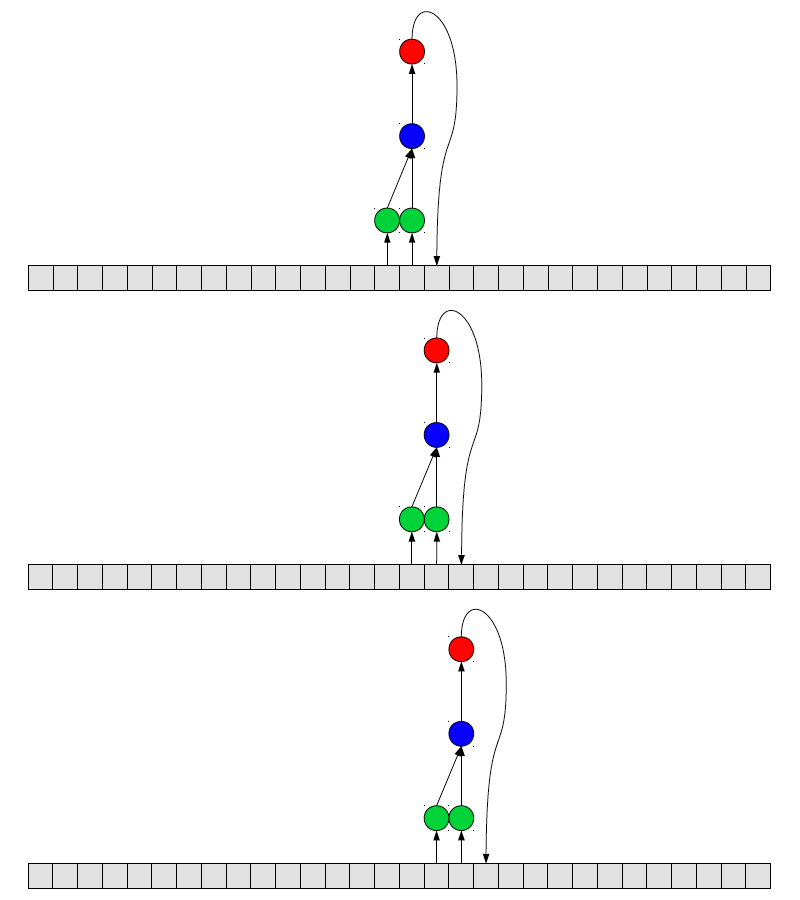
\includegraphics[width=0.8\textwidth]{pic02}
    \caption {Training of artificial neural sub-networks with 3-2-1 topology (left) and 4-2-1 topology (right).}
\label{fig:pic02}
\end{figure}
\FloatBarrier

Fourth sub-network has 4-2-1 topology and once again the size of the hidden layer is only illustrative (Fig. \ref{fig:pic02}-right). The real size of the hidden layer is estimated by incremental pruning algorithm. Training examples are one less than with the previous sub-network, because the input size is bigger by one. Training and stopping criteria are the same as with the previous sub-networks. Fig. \ref{fig:pic01} and \ref{fig:pic02} show only initial 4 sub-networks. In the model implementation many more sub-networks are involved. Sub-networks typologies are formed by addition of a single neuron in the input layer and adjustment of the hidden layer size with incremental pruning algorithm. The final goal is to reach n-m-1 topology (Fig. \ref{fig:pic03}), which covers all known time series values. Most of the links between the input and the hidden layers in Fig. \ref{fig:pic03} are missed for better visualization, but both layer are fully-connected in the model implementation. 

\begin{figure}[ht!]
   \centering
     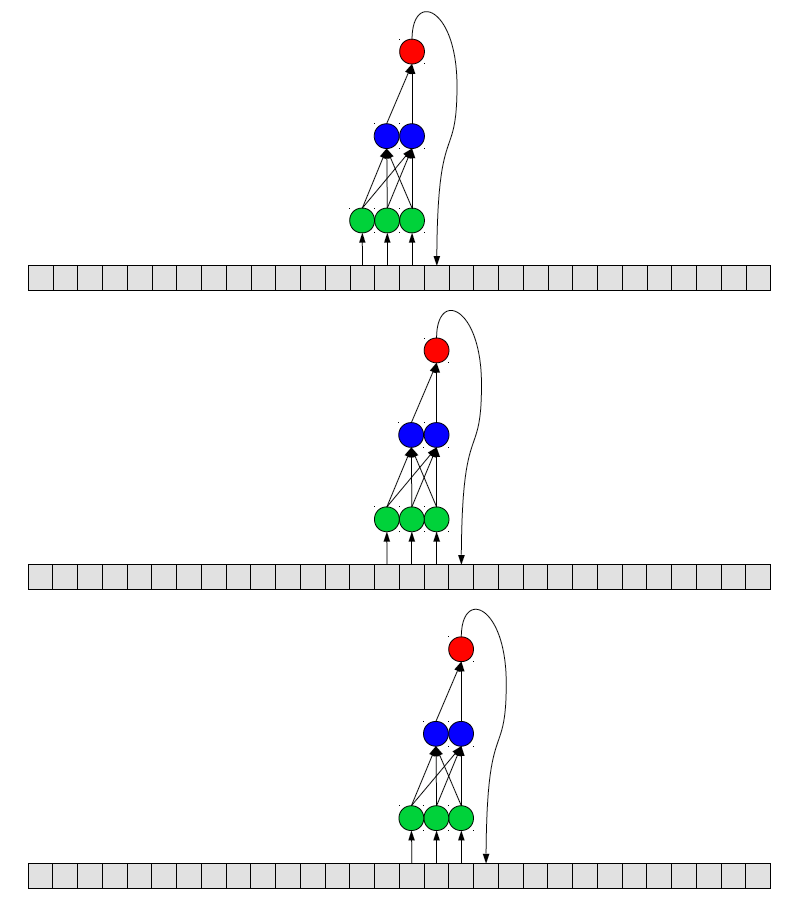
\includegraphics[width=0.8\textwidth]{pic03}
    \caption {Training of artificial neural sub-network with n-m-1 topology. Some of the links between input and hidden layer are not visualized for better appearance.}
\label{fig:pic03}
\end{figure}
\FloatBarrier

After the training of the biggest sub-network hierarchical procedure goes back in a loop to the smallest sub-network. Values of the weights from the biggest sub-network, which correspond to the links in the smaller sub-network, are taken and are loaded in the smallest sub-network. In a similar manner weights are taken from the biggest sub-network for the other sub-networks in combination with the weights of the previous smaller sub-network weights. For example, the sub-network with 4-2-1 topology will take some of its weights from 3-2-1 sub-networks, but links which are not presented into the smaller sub-network will be taken from the biggest sub-network. 

The common idea behind the proposed model is the incremental training of racing in size artificial neural networks. Such training is inspired by the natural neural systems where biological cells grow in number and form connections between each other. The common problem in artificial neural networks training is the size of the network. By splitting the biggest network in many smaller networks speed up of the training process is achieved. It is very well known in the time series forecasting field that the oldest measurements have the smallest impact for the forecast. The proposed model takes this fact into account and the oldest measurements are taken in the biggest sub-network, but they have relatively smaller impact in the final forecast. The proposed model has higher degree of self-adaptation, because when a new value in the time series appears the size of the artificial neural network grows, which means that training phase and operation phase are simultaneous.

\section{Experiments and Results} \label{Experiments and Results}

All experiments are done as Java program where the artificial neural networks are implemented with the API provided by Encog Machine Learning Framework \cite{heaton01}. All input neurons do not have activation function, because their task is only to supply the input signals into the hidden layer. The neurons in the hidden and the output layer are used with hyperbolic tangent function. Hyperbolic tangent is preferred instead of the sigmoid function, because it has symmetry against X axis. This symmetry helps for the training speed up when backpropagation training is used, because the output values of the neurons have positive and negative values. With the sigmoid function output of the neurons is only positive and negative signals (if they are needed) can be achieved only by negative weights. 

\begin{figure}[ht!]
   \centering
     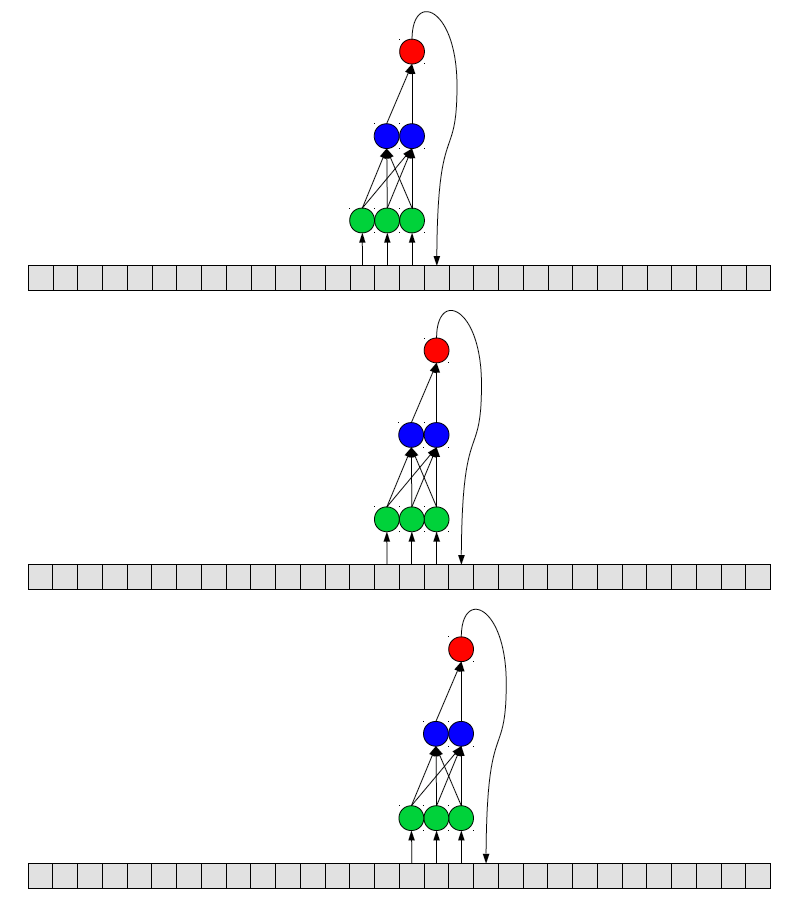
\includegraphics[width=0.8\textwidth]{pic04}
    \caption {Currencies values for two months on daily basis - EUR/USD currency pair.}
\label{fig:pic04}
\end{figure}
\FloatBarrier

As input data for the experiments FOREX financial time series are used (Fig. \ref{fig:pic04} and \ref{fig:pic05}). Date are taken for daily trading of two months for EUR/USD and USD/JPY currencies pairs. Time series values are scaled in the range of -0.99 to +0.99 with MinMax scaling rule. The output of the artificial neural network is re-scaled back to the original rage with the same rule, but used in the opposite direction. 

\begin{figure}[ht!]
   \centering
     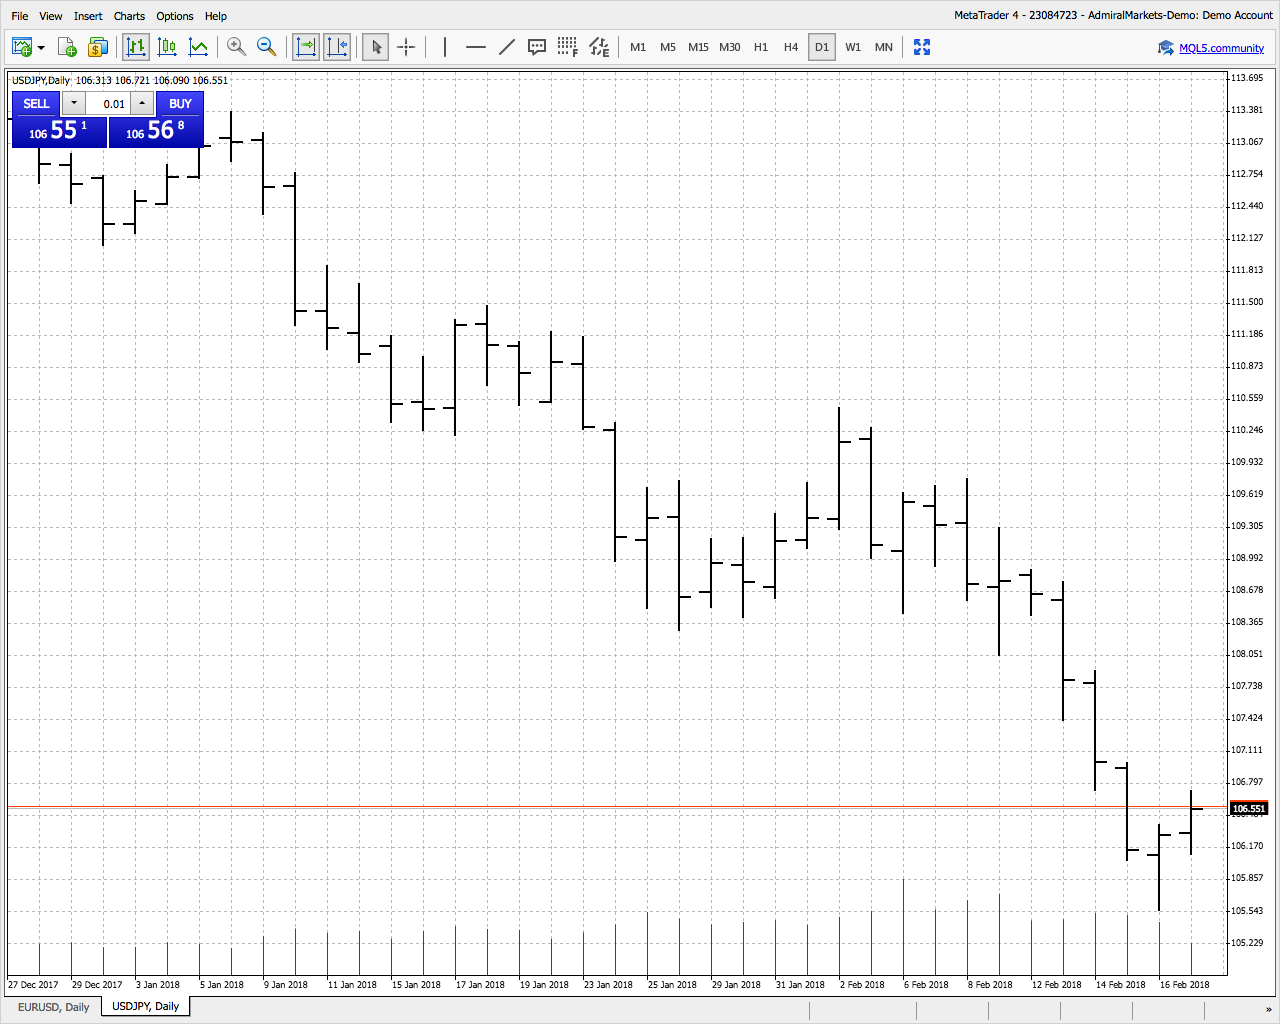
\includegraphics[width=0.8\textwidth]{pic05}
    \caption {Currencies values for two months on daily basis - USD/JPY currency pair.}
\label{fig:pic05}
\end{figure}
\FloatBarrier

The results of the experiments are still in the range of the statistical error, which comes from the complexity of the financial processes and the high-frequency noise inside the data. 

\section{Conclusion} \label{Conclusion}

The proposed model for self rising tri layers MLP for time series forecasting is a promising approach for artificial neural networks training speed-up. The rising size of the input layer involve a maximum information available in the time series, but the proposed procedure for artificial neural network training takes in account that older values should be less informative. As further research it will be interesting such self-rising training to be implemented az parallel computing solution. 

\begin{thebibliography}{99}

\bibitem{atanasova01} Atanasova T., Barova M., Exploratory analysis of Time Series for hypothesize feature values, Proceedings of International Scientific Conference UniTech17, Gabrovo, Bulgaria, ISSN: 1313-230X, 2017, V. 2, P. 399--403.

\bibitem{balabanov01} Balabanov, T., Zankinski, I., Dobrinkova, N., Time Series Prediction by Artificial Neural Networks and Differential Evolution in Distributed Environment, Proceedings of the International Conference on Large-Scale Scientific Computing, Sozopol, Bulgaria, Lecture Notes in Computer Science, Springer, ISBN 978-3-642-29842-4, 2011, V. 7116, N. 1, P. 198–-205. 

\bibitem{balabanov02} Balabanov, T., Long Short Term Memory in MPL Pair, Proceedings of the  International Scientific Conference UniTech17, Gabrovo, Bulgaria, ISSN: 1313-230X, 2017, V. 2, P. 375--379.

\bibitem{tashev01} Tashev T., Hristov H., Modeling of Synthesis of Information Processes with Generalized Nets, Cybernetics and Information Technologies, Academic Publishing House Prof. Marin Drinov, Sofia, Bulgaria, 2003, V.2, P. 92--104.

\bibitem{alexandrov01} Alexandrov, A., AD HOC Kalman filter based fusion algorithm for real-time Wireless Sensor Data Integration, Proceedings of the Eleventh International Conference Flexible Quering Answering Systems, Warsaw, Poland, Springer, ISBN 978-3-319-26153-9, 2015, V. 400, P. 151--160.

\bibitem{heaton01} Heaton J., Encog Machine Learning Framework, Heaton Research, Inc., \url{http://www.heatonresearch.com/encog/}

\end{thebibliography}

\end{document}
